\documentclass[main.tex]{subfiles}
\begin{document}



\chapter{Reihen}


\begin{Definition}
 Sei $(v_n)_{n=0}^\infty$ eine Folge in $\R$ (alternativ in einem normierten Vektorraum $(v,||.||)$) und $A \in \R$ (bzw. in $V$).
 $$\sum \limits_{n=0}^\infty v_n = A \Leftrightarrow \limn \sum \limits_{k=0}^n v_n = A \Leftrightarrow \A \varepsilon > 0 \E N \in \N : n \geq N \Rightarrow \left|\left| \sum \limits_{k=0}^n v_k -A \right|\right| < \varepsilon$$
 bedeutet,  (per Definition), dass $\sum \limits_{n=0}^\infty v_n = A$
\end{Definition}

\begin{Bemerkung}
  Eine Reihe ist außerdem per Definition die Summe aller Partialsummen:\\
  $$∑_{n=1}^\infty a_n = \lim \limits_{N → \infty} \underbrace{∑_{n=1}^N a_n}_{s_n}$$
\end{Bemerkung}

\begin{Theorem}
  $$∑_{k=1}^\infty a_k \text{ konvergiert } ⇔ \limn a_n = 0$$
\end{Theorem}

\begin{Lemma}
  Seien $\sum \limits_{k=1}^\infty a_k$, $\sum \limits_{k=1}^\infty b_k$ konvergente Reihen und $α,β ∈ \C$. Dann gilt
   $$∑_{k=1}^\infty (α a_k + β b_k) = α ∑_{k=1}^\infty a_k + β ∑_{k=1}^\infty b_k$$
   Insbesondere bilden konvergente Reihen einen Vektorraum über $\C$ und der Wert der Reihe stellt eine lineare Abbildung auf diesem Vektorraum nach $\C$ dar.
\end{Lemma}


\section{Konvergenz von Reihen}

\begin{Theorem}[Majoranten-/Minorantenkriterium]
   Seien $\sum \limits_{k=1}^\infty a_k$ und $\sum \limits_{k=1}^\infty b_k$ zwei Reihen mit der Eigenschaft $0 ≤ a_k ≤ b_k$ für alle$ k ∈ \N$. Dann gilt
   $$\sum \limits_{k=1}^\infty a_k \leq \sum \limits_{k=1}^\infty b_k$$
   und insbesondere gelten die Implikationen
   $$\sum \limits_{k=1}^\infty b_k \text{ konvergent } \Rightarrow  \sum \limits_{k=1}^\infty a_k \text{ konvergent }$$
   $$\sum \limits_{k=1}^\infty a_k \text{ divergent } \Rightarrow  \sum \limits_{k=1}^\infty b_k \text{ divergent }$$
   Diese beiden Implikationen treffen auch dann zu, wenn $0 ≤ a_n ≤ b_n$ nur für alle hinreichend großen $n ∈ \N$ gilt.
\end{Theorem}

\begin{Theorem}[Verdichtungskriterium]
  Sei $(a_n)_{n=0}^\infty$ eine monoton fallende Folge positiver reeller Zahlen. Dann gilt:
  $$∑_{n=0}^\infty a_n \text{ konvergiert } ⇔ ∑_{n=0}^\infty 2^na_{2^n} \text{ konvergiert}$$
\end{Theorem}

\begin{Theorem}[Leibnitz-Kriterium]
  Sei $(a_n)_{n=0}^\infty$ eine monoton fallende Folge positiver reeller Zahlen, die gegen Null konvergiert. Dann konvergiert die alternierende Reihe $∑_{k=0}^\infty (−1)^k a_k$ und es gilt
  $$∑_{k=0}^{2n−1} (−1)^k a_k \leq  ∑_{k=0}^\infty (−1)^k a_k ≤ ∑_{k=0}^{2n} (−1)^k a_k$$
  für alle $n ∈ \N$.
\end{Theorem}

\begin{Theorem}[Cauchy-Kriterium]
  Die Reihe komplexer Zahlen $\sum \limits_{k=1}^\infty a_k$ konvergiert genau dann, wenn es zu jedem $ε > 0$ ein $N ∈ \N$ gibt, so dass für $n ≥ m ≥ N$
  $$\left|∑_{k=m}^n a_k \right| < ε$$
  erfüllt ist.
\end{Theorem}

\begin{Beweis}
  Siehe Skript.
\end{Beweis}

\subsection{Absolute Konvergenzkriterien}

\begin{Definition}[Absolute Konvergenz]
  $$\sum \limits_{n=0}^\infty v_n \text{ konvergiert absolut } \Leftrightarrow \sum \limits_{n=0}^\infty |v_n| \text{ konvergiert}$$
\end{Definition}

\begin{Bemerkung}
  Wenn $v_n$ insbesondere nach oben beschränkt ist.
\end{Bemerkung}

\begin{Theorem}[Cauchy's Wurzelkriterium]
  Sei $(a_n)_{n=0}^\infty$ eine Folge komplexer Zahlen und
  $$α = \limsup_{n → \infty} \sqrt[n]{|a_n|} ∈ \R ∪ \{\infty\}$$
  Dan gilt
  $$α < 1 ⇒ ∑_{n=1}^\infty a_n \text{ konvergiert absolut.}$$
  $$α > 1 ⇒ ∑_{n=1}^\infty a_n \text{ divergiert.}$$
\end{Theorem}

\begin{Beweis}
  Angenommen $α < 1$. Dann gilt:
  $$\E n ∈ \N : \sup_{k \geq n} \sqrt[k]{|a_k|} < q = \dfrac{1+α}{2} < 1$$
  Und somit $|a_k| < q^k \A k \geq n$. Die Reihe konvergiert somit absolut nach dem Majorantenkriterium (und der Eigenschaft der geometrischen Reihe). Falls $\alpha > 1$ gilt, so gib es eine Teilfolge $(a_{n_k})_{k=0}^\infty$ mit $\sqrt[n_k]{|a_{n_k}|} > 1$ für alle $k$. Daraus folgt aber $|a_{n_k}| > 1$, und insbesondere ist $(a_n)_n$ keine Nullfolge und die entsprechende Reihe divergiert.
\end{Beweis}

\begin{Korollar}[D'Alembert's Quotientenkriterium]
  Sei $(a_n)_{n=0}^\infty$ eine Folge komplexer Zahlen mit $a_n \neq 0 \A n$. Setze
  $$\rho = \limsup_{n\to \infty}\left|\dfrac{a_{n+1}}{a_n}\right|$$
  \begin{itemize}
    \item Falls $\rho < 1$, dann konvergiert $\sum \limits_{n=0}^\infty a_n$ absolut.
    \item Falls $\rho > 1$, dann konvergiert $\sum \limits_{n=0}^\infty a_n$ nicht absolut. (aber sie divergiert nicht notwendigerweise und kann auch konvergieren.)
  \end{itemize}
\end{Korollar}

\begin{Beweis}
  \begin{itemize}
    \item Angenommen $\rho < 1$. Sei $\lambda \in (\rho,1)$, also $\rho < \lambda < 1$.\\
      Dann $\E N \in \N : n \geq N \Rightarrow \left| \dfrac{a_{n+1}}{a_n} \right| \leq \lambda$ (Definition des limsup!).\\
      Folgt: $|a_{N+1}| \leq \lambda |a_n| \Leftrightarrow |a_{N+2}| \leq \lambda^2 |a_n| \Leftrightarrow ... \Leftrightarrow |a_{N+k}| \leq \lambda^k |a_n|$
      $$\begin{aligned}
        \sum \limits_{n=0}^\infty |a_n| &= \sum \limits_{n=0}^{N-1} |a_n| + \sum \limits_{k=0}^\infty |a_{N+k}|\\
        &\leq \sum \limits_{n=0}^{N-1} |a_n| + |a_N|\cdot \sum \limits_{k=0}^\infty \lambda^k \\
        &< \infty
      \end{aligned}$$
      Der endliche Teil der Summe konvergiert sowieso, der 2. Teil auch, denn $\lambda <1$.
    \item (Falls $\rho > 1$, gilt: $\E N \in \N : n \geq N \Rightarrow |a_{n+1} \leq |a-n|s$.

      Insbesondere: $|a_{N+k}| \geq |a_N| > 0$, also $\limn a_n \neq 0$.

      Folgt: $\sum \limits_{n=0}^\infty a_n$ divergiert.)
  \end{itemize}
\end{Beweis}

\begin{Beispiel}
  Sei $a_n = \left\{\begin{aligned}
    10^{-n} & n \text{ gerade}\\
    2 \cdot 10^{-n} & n \text{ ungerade}
  \end{aligned}\right.$

  Also gilt: $$\limsup \left| \dfrac{a_{n+1}}{a_n} \right| = 2 > 1$$
  $$\sum \limits_{n=0}^\infty a_n = \sum \limits_{k=0}^\infty \dfrac{3}{10^{2k}}$$
\end{Beispiel}

\begin{Theorem}
  Sei $\sum \limits_{n=0}^\infty a_n$ eine absolut konvergierende Reihe (in $\R$, $\C$ oder jeglichem $(V,||.||)$). Sei $\varphi: \N \to \N$ eine Bijektion. Dann konvergiert $\sum \limits_{n=0}^\infty a_{\varphi(n)}$ ebenfalls absolut und es gilt:
  $$\sum \limits_{n=0}^\infty a_n = \sum \limits_{n=0}^\infty a_{\varphi(n)}$$
\end{Theorem}

\begin{Beweis}
  \begin{itemize}
    \item Absolute Konvergenz: Sei $\varepsilon > 0$, dann $\E N \in  \N : n \geq m \geq N \Rightarrow \sum \limits_{k=m}^n |a_k| < \varepsilon$.

      Sei $M \in \N$, so dass $n \geq M \Rightarrow \varphi(n) \geq N$.\\
      Für $n \geq m \geq M$ gilt dann:
      $$\sum \limits_{k=m}^n |a_{\varphi(n)}| \leq \sum \limits_{k=N}^l|a_k| < \varepsilon$$
      mit $l = \max\{\varphi(m),\varphi(m+1),...,\varphi(n)\}$
    \item Selbes Argument für die Gleichheit der Grenzwerte (wird dem Leser als Übung gelassen).
  \end{itemize}
\end{Beweis}

\begin{Korollar}
  Seien $\sum \limits_{n=0}^\infty a_n$ und $\sum \limits_{n=0}^\infty b_n$ absolut konvergierend uns sei $\psi : \N \to \N^2$ eine Bijektion: $\psi(n) = (\phi(n),\eta(n))$
  $$\left(\sum \limits_{n=0}^\infty a_n\right) \cdot \left(\sum \limits_{n=0}^\infty b_n\right) = \sum \limits_{n=0}^\infty a_{\phi(n)} b_{\eta(n)}$$
\end{Korollar}

\begin{Beweis}
  Wir betrachten folgende (spezielle) Bijektion $\psi : \N \to \N^2$
  Es gilt: $\psi(0) = (0,0), \psi(1)=(1,0), \psi(2) = (1,1), \psi(3) = (0,1), \psi(4) = (-1,1),...$ Man formt also wachsende Quadrate:

  \begin{center}
    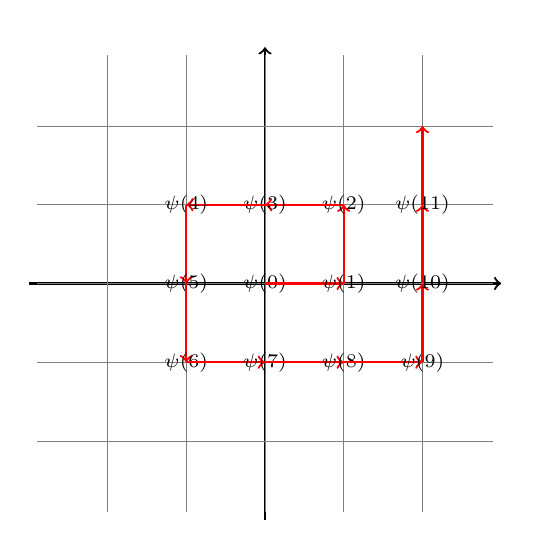
\begin{tikzpicture}
      \draw[thick,->] (-3,0) -- (3,0) node[anchor=north west] {$\N$};
      \draw[thick,->] (0,-3) -- (0,3) node[anchor=south east] {$\N$};
      \draw[step=1cm,gray,very thin] (-2.9,-2.9) grid (2.9,2.9);

      \draw (0,0) node {$\scriptstyle \psi(0)$};
      \draw[->,red,thick] (0,0) -- (1,0);
      \draw (1,0) node {$\scriptstyle \psi(1)$};
      \draw[->,red,thick] (1,0) -- (1,1);
      \draw (1,1) node {$\scriptstyle \psi(2)$};
      \draw[->,red,thick] (1,1) -- (0,1);
      \draw (0,1) node {$\scriptstyle \psi(3)$};
      \draw[->,red,thick] (0,1) -- (-1,1);
      \draw (-1,1) node {$\scriptstyle \psi(4)$};
      \draw[->,red,thick] (-1,1) -- (-1,0);
      \draw (-1,0) node {$\scriptstyle \psi(5)$};
      \draw[->,red,thick] (-1,0) -- (-1,-1);
      \draw (-1,-1) node {$\scriptstyle \psi(6)$};
      \draw[->,red,thick] (-1,-1) -- (0,-1);
      \draw (0,-1) node {$\scriptstyle \psi(7)$};
      \draw[->,red,thick] (0,-1) -- (1,-1);
      \draw (1,-1) node {$\scriptstyle \psi(8)$};
      \draw[->,red,thick] (1,-1) -- (2,-1);
      \draw (2,-1) node {$\scriptstyle \psi(9)$};
      \draw[->,red,thick] (2,-1) -- (2,0);
      \draw (2,0) node {$\scriptstyle \psi(10)$};
      \draw[->,red,thick] (2,0) -- (2,1);
      \draw (2,1) node {$\scriptstyle \psi(11)$};
      \draw[->,red,thick] (2,1) -- (2,2);
    \end{tikzpicture}
  \end{center}

  Sei $\varepsilon > 0$ und sei $N \in \N$ mit
  $$\sum \limits_{k=N}|a_k| < \varepsilon \text{ und } \sum \limits_{k=N}^\infty|b_k| < \varepsilon$$
  Jetzt gilt:
  $$\begin{aligned}
    \left(\sum \limits_{k=0}^\infty |a_k| \right) \cdot \left(\sum \limits_{l=0}^\infty |b_l|\right) &=
    \left(\underbrace{\sum \limits_{k=0}^{N-1} |a_k|}_{=A}
    + \underbrace{\sum \limits_{k=N}^\infty |a_k|}_{=\alpha}\right)
    \cdot \left(\underbrace{\sum \limits_{l=0}^{N-1} |b_l|}_{=B}
    + \underbrace{\sum \limits_{l=N}^\infty |b_l|}_{=\beta}\right)\\
    &= \sum \limits_{k=0}^{N-1}\sum \limits_{l=0}^{N-1}|a_k|\cdot|b_l| + \alpha B + \beta A + \alpha \beta\\
    &= \sum \limits_{n=0}^{(N-1)^2-1} |a_{\varphi(n)}|\cdot|b_{\eta(n)}| + \underbrace{\alpha B + \beta A + \alpha \beta}_{\to 0 \text{ mit } \varepsilon \to 0}
  \end{aligned}$$
  Ist $\psi':\N \to \N^2$ eine beliebige Bijektion, so gilt: $\psi' = \psi \circ \omega$ für eine Bijektion $\omega: \N \to \N$, $\omega = \psi^{-1}\psi'$.

  Also kann der Umformungssatz angewendet werden.
\end{Beweis}

\begin{Beispiel}
  \begin{itemize}
    \item Komplex:
      $$\sum \limits_{n=0}^\infty \dfrac{\sin(n)}{n^2}$$
    \item Machbar:
      $$\sum \limits_{n=0}^\infty \dfrac{n}{2^n}$$
      $$\rho = \limn \dfrac{\frac{n+1}{2^{n+1}}}{\frac{n}{2^n}} = \limn \dfrac{(n+1)2^n}{n \cdot 2^n} = \dfrac{1}{2} \limn \dfrac{n+1}{n} = \dfrac{1}{2}$$
      $\rho < 1 \Rightarrow$ die Reihe konvergiert absolut.

      Berechnung:
      $$\begin{aligned}
        \sum \limits_{n=1}^\infty \dfrac{n}{2^n}
        &= \sum \limits_{n=1}^\infty \underbrace{\left(\dfrac{1}{2^n} + ... + \dfrac{1}{2^n}\right)}_{n \text{ Mal}}\\
        &= \sum \limits_{n=1}^\infty \left(\sum \limits_{p=1}^n \dfrac{1}{2^p} \cdot \dfrac{1}{2^{n-p}}\right)\\
        &= \sum \limits_{n=1}^\infty \sum \limits_{p + q = n} \dfrac{1}{2^p} \cdot \dfrac{1}{2^q}\\
        &= \sum \limits_{p=1}^\infty \sum \limits_{q=0}^\infty \dfrac{1}{2^p} \cdot \dfrac{1}{2^q}\\
        &= \underbrace{\sum \limits_{p=1}^\infty \dfrac{1}{2^p}}_{= (1/2)/(1-1/2)} \cdot \underbrace{\sum \limits_{q=0}^\infty \dfrac{1}{2^q}}_{= 2}\\
        &= 2
    \end{aligned}$$
  \end{itemize}
\end{Beispiel}


\section{Potenzreihen}

\begin{Definition}[Potenzreihe]
  Sei $K$ ein Körper. Eine Potenzreihe (formale Potenzreihe) mit Koeffizienten in $K$ ist eine Folge $(a_n)_{n=0}^\infty$ in $K$, geschrieben als:
  $$\sum \limits_{n=0}^\infty a_k T^k$$
  mit $T$ als 'Variable'.\\
  Wir schreiben $K[\![T]\!]$ für die Menge aller formalen Potenzreihen.Für die Polynome $K[T]$ gilt $K[T] \subseteq K[\![T]\!]$

  Außerdem gilt:
  \begin{itemize}
    \item $0 = \sum \limits_{k=0}^n 0 \cdot T^k$
    \item $1 = 1 + \sum \limits_{k=0}^n 0 \cdot T^k$
    \item + (lästig)
    \item * (lästig)
  \end{itemize}
  ...$K[\![T]\!]$ ist ein \textbf{Ring}. (aber kein Körper, weil das multiplikative Inverse im Allgemeinen nicht existiert)
\end{Definition}

\begin{Bemerkung}
  Im Folgenden betreiben wir reelle Analysis, also werden wir $K = \R$ oder $K = \C$ wählen. Damit werden diese Polynome zu Reihen.
\end{Bemerkung}

\begin{Definition}[Konvergenzradius]
  Sei $\sum \limits_{n=0}^\infty a_n \cdot T^n \in \C[\![T]\!]$ und definiere
  $$\rho = \limsup_{n\to \infty} \sqrt[n]{|a_n|} \quad \in [0,\infty]\cup \{\infty\}$$
  Der Konvergenzradius von $\sum \limits_{n=0}^\infty a_n \cdot T^n$ ist
  $$R = \left\{ \begin{aligned}
    \infty & \text{ falls } \rho = 0 \\
    \dfrac{1}{\rho} & \text{ falls } \rho > 0, \rho \neq \infty \quad \in  [0,\infty]\\
    0 & \text{ falls } \rho = \infty
  \end{aligned}\right.$$
\end{Definition}

\begin{Beispiel}
  \begin{itemize}
    \item $\sum \limits_{n=0}^\infty T^n$, also $a_n = 1 \A n \in \N$\\
      $\rho = \limsup \sqrt[n]{|1|} = 1, R = \dfrac{1}{1} = 1$
    \item $\sum \limits_{n=0}^\infty \dfrac{1}{(n!)^2} T^n$\\
      $\rho = \limsup \sqrt[n]{|(n!)^{-2}|} = 0, R = \infty$
  \end{itemize}
\end{Beispiel}

\begin{Bemerkung}
  \begin{Theorem}
    Sei $\sum \limits_{n=0}^\infty a_n \cdot T^n$ eine formale Potenzreihe mit Konvergenzradius $R > 0$ und sie $z \in \C : |z| < R$. Dann konvergiert $\sum \limits_{n=0}^\infty a_n \cdot z^n$ absolut.
  \end{Theorem}
  \begin{Beweis}
    Grund dafür ist \textbf{Cauchy's Wurzelkriterium}:
    $$\limsup_{n\to\infty} \sqrt[n]{|a_n \cdot z^n|} = \limsup_{n\to\infty} \sqrt[n]{|a_n| \cdot |z^n|} = \limsup_{n\to\infty} \sqrt[n]{|a_n|} \cdot |z| = |z| \cdot \rho < 1$$
  \end{Beweis}
  \begin{minipage}{0.5\textwidth}
    \incfig{konvergenzradius}
  \end{minipage}
  \begin{minipage}{0.5\textwidth}
    $$\color{blue} \sum \limits_{n=0}^\infty a_n \cdot z^n \text{ konvergiert}$$
    $$\color{red} \sum \limits_{n=0}^\infty a_n \cdot z^n \text{ divergiert}$$
    $$\color{yellow} \sum \limits_{n=0}^\infty a_n \cdot z^n \text{ undefiniert}$$
  \end{minipage}
\end{Bemerkung}

\begin{Lemma}
  Sei $\sum \limits_{n=1}^\infty a_n T^n$ eine Potenzreihe mit $a_n \neq 0 \A n\in N$. Der Konvergenzradius $R$ ist gegeben durch
  $$R = \limn \dfrac{|a_n|}{a_{n+1}}$$
  falls dieser Grenzwert exisitiert.
\end{Lemma}
\begin{Beweis}
  Aufgabe.
\end{Beweis}

\begin{Beispiel}
  $$\sum \limits_{n=0}^\infty \dfrac{z^n}{n}, \text{ also } a_n = \dfrac{1}{n}$$
  $$\rho = \limsup_{n \to \infty} \sqrt[n]{\dfrac{1}{n}} = 1, R = 1$$
  \begin{itemize}
    \item $z = -1 \Rightarrow \sum \limits_{n=1}^\infty \dfrac{(-1)^n}{n}$ konvergiert
    \item $z = 1 \Rightarrow \sum \limits_{n=1}^\infty \dfrac{1}{n}$ divergiert
    \item $z = i \Rightarrow$ divergiert (kann unter Verwendung des Leibnitzkriteriums für $Re$ und $Im$ gezeigt werden.)
  \end{itemize}
\end{Beispiel}

\begin{Lemma}
  Seien $D \subseteq \R$, $f_n: D \to \R$, $n \in \N$, $f: D \to \R$.\\
  Angenommen $f_n$ ist stetig $\A n$ und $\A \varepsilon > 0 \E N \in \N$ mit
  $$||f_n - f||_\infty < \varepsilon \A n \geq N$$
  d.h. $\limn f_n = f$ bezüglich $||.||_\infty$.\\
  Dann ist $f$ \textbf{ stetig}. Man sagt $(f_n)_{n=0}^\infty$ konvergiert gleichmäßig gegen $f$.
\end{Lemma}

\begin{Bemerkung}
  Diese Behauptung kann analog auf $\C$ erweitert werden.
\end{Bemerkung}

\begin{Beweis}
  \begin{itemize}
    \item Stetigkeit von $f$: Sei $x_0 \in D$, $\varepsilon > 0$. Es existiert also ein $n \in \N : ||f-f_n|| < \underbrace{\varepsilon \cdot \frac{1}{3}}_{\text{Kosmetik}}$.\\
      Das heißt $|f(x)-f_n(x)| < \dfrac{\varepsilon}{3} \A x \in D$\\
      $f_n$ ist stetig: $$\E \delta > 0 : |x - x_0| < \delta \Rightarrow |f_n(x) - f_n(x_0)| < \dfrac{\varepsilon}{3}$$
      Folgt: für $x \in D$ mit $|x - x_0| < \delta$:
      $$\begin{aligned}
      |f(x)-f(x_0)| &= |f(x) -f_n(x) + f_n(x) - f_n(x_0) + f_n(x_0) - f(x_0)|\\
      &\leq \underbrace{|f(x)-f_n(x)|}_{\leq \varepsilon/3} + \underbrace{|f_n(x) - f_n(x_0)|}_{\leq \varepsilon/3} + \underbrace{|f_n(x_0) - f(x_0)|}_{< \varepsilon/3}\\
      &< \varepsilon
      \end{aligned}$$
  \end{itemize}
\end{Beweis}

\begin{Theorem}
  Sei $\sum \limits_{n=0}^\infty a_n \cdot T^n \in \C[\![T]\!]$ eine Potenzreihe mit Konvergenzradius $R > 0$. Sei $r > 0$, $r < R$, und schreibe $D = B(0,r) \subseteq \C$ und definiere $f_n: D \to \C$ durch
  $$f_n(z) = \sum \limits_{k=0}^n a_k \cdot z^k \quad \text{stetig da Polynomfunktion}$$
  Für $z \in D$ definiere:
  $$f(z) = \sum_{k=0}^\infty a_k \cdot z^k \quad \text{konvergiert absolut}$$
  Dann gilt:

  Die Folge $(f_n)_{n=0}^\infty$ konvergiert \textbf{gleichmäßig} gegen $f$. Insbesondere gilt: $f$ ist stetig.\\
  Ausgeschrieben:
  $$\A \varepsilon > 0 \E N \in \N : n \geq N \Rightarrow \left|f(z) - \sum \limits_{k=0}^\infty a_k \cdot z^k \right| < \varepsilon \A z \in D$$
\end{Theorem}

\begin{Beweis}
  Für $z \in D$ konvergiert $\sum \limits_{k=0}^\infty |a_k| \cdot r^k$. Also:
  $$\A \varepsilon > 0 \E N \in \N : \sum \limits_{k=N}^\infty |a_k| \cdot r^k < \varepsilon$$
  Folgt:
  $$\A z \in D : \left|f(z) - \sum \limits_{k=0}^n a_k \cdot z^k \right| = \left|\sum \limits_{k=n+1}^\infty a_k \cdot z^k \right| \leq \sum \limits_{k=n+1}^\infty |a_k| \cdot |z^k| \leq \sum \limits_{k=n+1}^\infty |a_k| \cdot r^k < \varepsilon$$
\end{Beweis}


\section{Integration von Reihen}

\subsection{Potenzreihen}

\begin{Lemma}
  Sei $[a,b] \subseteq \R$ mit $a < b$. Seien $(f_n)_{n=0}^\infty$ eine Folge stetiger Funktionen auf $[a,b]$, $f:[a,b] \to \R$ stetig mit $\limn f_n = f$ bezüglich $||.||_\infty$. Dann gilt:
  $$\limn \int_a^b f_n dx = \int_a^b f dx$$
  \begin{Bemerkung}
    Dank der spezifischen Hypothesen des Lemmas kann man anschaulich die Grenzwerte vertauschen (das Integral ist der Grenzwert der Treppenfunktionen).
  \end{Bemerkung}
\end{Lemma}

\begin{Beweis}
  Sei $\varepsilon > 0$.
  $$\E N \in \N : ||f - f_n||_\infty < \varepsilon \A n \geq N$$
  $$\Leftrightarrow |f(x)- f_n(x) < \varepsilon \A x \in [a,b], n \geq N$$
  $$\Rightarrow \int_a^b|f(x)-f_n(x)|dx \leq \varepsilon \cdot (b-a)$$
  $$\Rightarrow \left|\int_a^b f_n dx - \int_a^b dx \right| < \varepsilon \cdot (b-a)$$
  Zur kosmetik können wir Anfangs $\varepsilon/(b-a)$ wählen.
\end{Beweis}

\begin{Korollar}
  Sei $\sum \limits_{n=0}^n a_n \cdot T^n \in \R[\![T]\!]$ eine Potenzreihe mit konvergenzradius $R > 0$. Seien $a,b \in \R$, $-R < a < b < R$.\\
  Definiere $f:[a,b] \to \R$ durch
  $$f(x) = \sum \limits_{n=0}^\infty a_n x^n \text{ (bewiesenermaßen stetig)}$$
  Definiere $F:[a,b] \to \R$ durch
  $$F(x) = \sum \limits_{n=0}^\infty \dfrac{a_n}{n+1}a_n x^{n+1} \text{ (bewiesenermaßen stetig)}$$
  Dann gilt:
  $$\int_a^b f(x)dx = F(b) - F(a)$$
\end{Korollar}

\begin{Beweis}
  Setze $f_n(x) = \sum \limits_{k=0}^n a_k x^k$. $f_n$ ist eine Polynomfunktion also insbesondere stetig und es gilt $(f_n)_{n=0}^\infty \to f$ (konvergiert) gleichmäßig.\\
  Folgt dank Lemma:
  $$\begin{aligned}
    \limn \int_a^b f_n dx &= \int_a^b f(dx)\\
    &= \limn \sum \limits_{k=0}^n a_k \int_a^b x^k dx \\
    &= \limn \sum \limits_{k=0}^n a_k \dfrac{1}{k+1} b^{k+1}\\
    &= \sum \limits_{k = 0}^\infty a_k \dfrac{b^k}{k+1} - \sum \limits_{k=0}^\infty a_k \dfrac{a^k}{k+1}\\
    &= F(b) - F(a)
  \end{aligned}$$
\end{Beweis}

\begin{Bemerkung}
  Das bedeutet, dass wir eine Funktion integrieren können, sobald wir sie als Potenzreihe darstellen können.
\end{Bemerkung}

\begin{Theorem}[Abel'scher Grenzwertsatz]
  Sei $\sum \limits_{n=0}^\infty a_n T^n \in \C[\![T]\!]$ mit Konvergenzradius $R > 0, R \in \R$.\\
  Angenommen $\sum \limits_{n=0}^\infty a_n R^n$ konvergiert. Dann gilt
  $$ \lim \limits_{\substack{t \to R \\ t < R}} \sum \limits_{n=0}^\infty a_n t^n = \sum \limits_{n=0}^\infty a_n R^n$$
  Mit anderen Worten: Die Funktion $f:(-R,R]$ definiert durch
  $$f(t) = \sum \limits_{n=0}^\infty a_n t^n$$
  ist stetig (bei $R$).
\end{Theorem}

\begin{Beweis}
  Wir ersetzen $a_n$ durch $a_n \cdot R^n$ und können damit annehmen, $R = 1$
  Für $0 \leq t < 1$ setze $f(t) = \sum \limits_{n=0}^\infty a_n t^n$. Also $f:[0,1) \to \C$ ist stetig.\\
  Betrachte
  $$\begin{aligned}
    \dfrac{1}{1-t}f(t) &= \left(\sum \limits_{n=0}^\infty t^n\right)\left(\sum \limits_{n=0}^\infty a_n t^n\right) \\
    &= \sum \limits_{n=0}^\infty \underbrace{(a_0 + a_1 + ... + a_n)}_{ = A_n} t^n
  \end{aligned}$$
  $$A = \limn A_n = \sum \limits_{n=0}^\infty a_n \cdot 1^n$$
  Ziel: $\lim \limits_{\substack{t \to 1 \\ t < 1}} f(t) = A$.

  Sei $\varepsilon > 0$. Setze $b_n = A_n - A$
  $$\begin{aligned}
    f(t) &= (1-t) \sum \limits_{n=0}^\infty A_n t^n\\
    &= (1-t) \sum \limits_{n=0}^\infty (b_n + A) t^n\\
    &= (1-t) \sum \limits_{n=0}^\infty b_n t^n + \underbrace{(1-t) \sum \limits_{n=0}^\infty A t^n}_{= A}
  \end{aligned}$$
  Es existiert $N \geq 0$ mit $n \geq N \Rightarrow |b_n| < \varepsilon$.
  $$\begin{aligned}
    |f(t)-A| & \leq \underbrace{\left|(1-t) \sum \limits_{n=0}^N b_n t^n\right|}_{:= P(t)} + \left|(1-t) \sum \limits_{n=N+1}^\infty b_n t^n\right|\\
    & \leq |P(t)| + \underbrace{(1-t) \sum \limits_{n=0}^\infty \varepsilon t^n}_{ = \varepsilon}
  \end{aligned}$$
  $$|f(t)-A| \leq |P(t)| + \varepsilon \text{ (weil $P$ stetig und $P(1) = 0$)}$$
  Also:
  $$\E \delta > 0 : t \in (1-\delta, 1) \Rightarrow |P(t)| < \varepsilon$$
  Folgt: Für $t \in (1-\delta, 1)$ gilt $|f(t)-A| < 2 \varepsilon \Rightarrow f(t)$ konvergiert gegen $A$.
  \begin{Bemerkung}
    Die Kosmetik, um auf $\varepsilon$ zu kommen wird dem Leser überlassen.
  \end{Bemerkung}
\end{Beweis}


\section{Exponentialfunktion (2. Ansatz)}

\begin{Definition}[Exponentialreihe]
  Wir bezeichnen die formale Potenzreihe
  $$\sum \limits_{n = 0}^\infty \dfrac{T^n}{n!} \quad \in \C [\![T]\!]$$
  als \textbf{Exponentialreihe}.

  Diese hat folgende Eigenschaften:
  \begin{Theorem}
    $$\rho = \limsup_{n \to \infty} \sqrt[n]{\dfrac{1}{n!}} = 0 \Rightarrow R = \infty$$
    $$\Rightarrow \sum \limits_{n=0}^\infty \dfrac{z^n}{n!} \text{ konvergiert absolut für alle $z \in \C$}$$
    $$\text{Die Funktion } f: \C \to \C, f(z) = \sum \limits_{n=0}^\infty\dfrac{z^n}{n!} \text{ ist stetig}$$
  \end{Theorem}
\end{Definition}

\begin{Theorem}
  Sei $t\in \R$. Dann gilt:
  $$\exp(t) = \limn \left(1 + \dfrac{t}{n}\right)^n = \sum \limits_{n=0}^\infty \dfrac{z^n}{n!}$$
\end{Theorem}

\begin{Beweis}
  Klassische Beweisskizze im Skript.

  Zu zeigen: $f(t)$ erfüllt die Funktionalgleichungen der Exponentialfunktion.
  \begin{itemize}
    \item $f(0) = 1$ \checkmark
    \item $f(x+y) = f(x)f(y)$ Nachrechnen (Kombinatorik) \checkmark
    \item $f(-x) = f(x)^{-1}$ HOW?
    \item $f(t) > 0 \A t \in \R$ \checkmark
    \item Zeige: $f(t) \geq 1+t$\\
      Für $t \geq 0$ gilt: $f(t) = 1 + \dfrac{t^1}{1!} + \underbrace{ ... }_{\geq 0} \Rightarrow f(t) \geq 1+t$\\
      Für $T \in (-1,0)$ gilt: $f(t) = 1 + \dfrac{t}{1} + \dfrac{t^2}{2} + \dfrac{t^3}{6} + ... \Rightarrow \text{ (Leibnitz) } 1+t \leq f(t) ( \leq 1 + t + \dfrac{t^2}{2})$
  \end{itemize}
  $$\Rightarrow f = \exp$$
\end{Beweis}

\begin{Bemerkung}
  Wir haben somit die Definition unserer Funktion von $\R \to \R$ auf $\C \to \C$ ausgeweitet. Für $t\in \R$ erhalten wir die bekannten Eigenschaften, für $t \in \C$ erhalten wir neue Eigenschaften (hint: Trigonometrie).
\end{Bemerkung}

\begin{Korollar}
  Für $a < b \in \R$ gilt:
  $$\int_a^b \exp(x) dx = \exp(b) - \exp(a)$$
\end{Korollar}

\begin{Theorem}
  Seien $z,w \in \C$, dann gilt:
  \begin{enumerate}
    \item $\exp(z+w) = \exp(z)\cdot \exp(w)$
    \item $|\exp(z)| = \exp(Re(z))$
  \end{enumerate}
  Insbesondere gilt: $|\exp(i \cdot t)| = 1 \A t \in \R$
\end{Theorem}

\begin{Beweis}
  \begin{enumerate}
    \item
        $$\begin{aligned}
        \exp(z)\cdot \exp(w) &=
        \sum \limits_{p=0}^\infty \dfrac{w^p}{p!} \cdot \sum \limits_{q=0}^\infty \dfrac{z^q}{q!}\\
        &= \sum \limits_{p=0}^\infty \sum \limits_{q=0}^\infty \dfrac{w^p}{p!} \cdot \dfrac{z^q}{q!}\\
        &= \sum \limits_{n=0}^\infty \underbrace{\sum \limits_{p=0}^\infty \dfrac{w^p z^{n-p}}{p!(n-p)!} \cdot \dfrac{n!}{n!}}_{= \dfrac{1}{n!} \sum \limits_{p=0}^\infty w^p z^{n -p} {n \choose p} = \dfrac{1}{n!}(w+z)^n}\\
        &= \sum \limits_{n=0}^\infty \dfrac{(w+z)^n}{n!}\\
        &= \exp(w+z)
      \end{aligned}$$
    \item Es gilt:\\
      \begin{minipage}{0.45\textwidth}
        $$\begin{aligned}
          \exp(\overline{z}) &= \sum \limits_{n=0}^\infty \dfrac{\overline{z}^n}{n!}\\
          &= \overline{\sum \limits_{n=0}^\infty \dfrac{z^n}{n!}}\\
          &= \overline{\exp(z)}
        \end{aligned}$$
      \end{minipage}
      \begin{minipage}{0.45\textwidth}
        Außerdem:
        $$\begin{aligned}
          |\exp(z)|^2 &= \exp(z)\exp(\overline{z})\\
          &= \exp(z + \overline{z})\\
          &= \exp(2\cdot Re(z))\\
          &= \exp(Re(z))^2
      \end{aligned}$$
      \end{minipage}
  \end{enumerate}
\end{Beweis}

\subsection{Trigonometrische Funktionen}

\begin{Definition}
  Für $z \in \C$ schreiben wir:
  $$\sin(z) = \sum \limits_{n=0}^\infty \dfrac{(-1)^n}{(2n+1)!} z^{2n+1}$$
  $$\cos(z) = \sum \limits_{n=0}^\infty \dfrac{(-1)^n}{(2n)!} z^{2n}$$
  $\sin,\cos: \C \to \C$ sind stetig (ebenfalls für $\R \to \R$)
  \begin{Theorem}
    Es gilt $\A z \in \C$:
    \begin{itemize}
      \item $\cos(-z) = \cos(z)$
      \item $\sin(z) = -\sin(z)$
    \end{itemize}
  \end{Theorem}
\end{Definition}

\begin{Theorem}
  Sei $z \in \C$. Dann gilt
  \begin{itemize}
    \item $\exp(i\cdot z) = \cos(z) + i \cdot \sin(z)$
    \item $\sin(z) = \dfrac{\exp(iz) - \exp (-iz)}{2i}$
    \item $\cos(z) = \dfrac{\exp(iz) + \exp (-iz)}{2}$
  \end{itemize}
  Insbesondere gilt für $z,w \in \C$:
  \begin{itemize}
    \item $\sin(z+w) = \sin(z)\cos(w) + \cos(z)\sin(w)$
    \item $\cos(z+w) = \cos(z)\cos(w) - \sin(z)\sin(w)$
  \end{itemize}
\end{Theorem}

\begin{Beweis}
  \begin{itemize}
    \item Zusammenhang sin,cos, exp:
      $$\begin{aligned}
        \exp(iz) = \sum \limits_{n=0}^\infty \dfrac{(iz)^n}{n!} &= 1 + \dfrac{iz}{!} + \dfrac{-z^2}{2!} + \dfrac{-iz^3}{3!} + \dfrac{z^4}{4!} + ... \\
        &= \sum \limits_{n=0}^\infty \dfrac{(-1)^nz^{2n}}{(2n)!} + i \sum \limits_{n=0}^\infty \dfrac{(-1)^nz^{2n+1}}{(2n+1)!}\\
        &= \cos(z) + i \sin(z)
      \end{aligned}$$
    \item Alternative Darstellung von sin, cos:
      $$\begin{aligned}
        \exp(iz) - \exp(-iz) &= \cos(z) + i \sin(z) - (-\cos(-z) - i \sin(-z))\\
        &= i \sin(z) + i \sin(z)\\
        &= 2i \sin(z)
      \end{aligned}$$
      Analog für $\cos$ kommt man auf die zweite Darstellung beider Funktionen.
    \item Additionstheoreme:
      $$\begin{aligned}
        \cos(z+w) + i \sin(z+w) & = \exp (iz + iw)\\
        & = \exp(iz) \cdot \exp(iw) \\
        & = (\cos(z) + i \sin(z))(\cos(w)+i\sin(w))\\
        & = \cos(z)\cos(w) - \sin(z)\sin(w)\\
        & + i (\sin(z)\cos(w) + \cos(z)\sin(w))\\
        & = \cos(z)\cos(w) - \sin(z)\sin(w)
      \end{aligned}$$
      Es lässt sich somit folgern:
      \begin{Theorem}[Kreisgleichung]
        $$1 = \\cos(0) = \\cos(z)^2 + \sin(z)^2$$
      \end{Theorem}
  \end{itemize}
\end{Beweis}

\begin{Theorem}
  Es existiert genau eine reelle Zahl $π \in (0,4)$ mit $\sin(π) = 0$. Für diese Zahl gilt:
  $$\exp(2π i) = 1$$
  Oder in \textbf{schön}:
  $$e^{i π} + 1 = 0$$
\end{Theorem}

\begin{Beweis}
  Für $x ∈ (0,2)$ sind die Folgen
  $$\left(\dfrac{x^{2n}}{(2n)!}\right)_{n=0}^\infty \text{ und } \left(\dfrac{x^{2n+1}}{(2n+1)!}\right)_{n=0}^\infty$$
  monoton fallend mit Grenzwert $0$.\\
  Also können wir beide mit Partialsummen abschätzen.\\
  Folgt:
  $$\dfrac{x}{1} -\dfrac{x^3}{6} < \sin(x) < \dfrac{x}{1} - \dfrac{x^3}{6} + \dfrac{x^5}{120} \text{ und } 1 - \dfrac{x^2}{2} < \cos(x) < 1 -\dfrac{x^2}{2} + \dfrac{x^4}{24}$$
  für $x \in (0,2)$.\\
  Wir wissen:
  \begin{itemize}
    \item $\dfrac{1}{\sqrt{2}} < 1 - \dfrac{1}{6} < \sin(1)$
    \item $\sin(0) = 0$
  \end{itemize}
  Also existiert laut Zwischenwertsatz ein $p \in (0,1)$ mit $\sin(p) = \dfrac{1}{\sqrt{2}}$.\\
  Setze $\pi = 4p$.\\
  Laut Kreisgleichung gilt: $\cos(p) = \sqrt{1 - \left(\dfrac{1}{\sqrt{2}}\right)^2} = \dfrac{1}{\sqrt{2}}$ (, was koherent ist mit der Aussage, das $\cos(x) > 0$ für $x \in (0,1)$).\\
  Jetzt gilt folgendes:
  \begin{itemize}
    \item $\exp(i p) = \dfrac{1+i}{\sqrt{2}}$
    \item $\exp(i \pi) = \exp(4 i p) = \dfrac{(1+i)^4}{4} = -1 = \underbrace{\cos(\pi)}_{=-1} + i \underbrace{\sin(\pi)}_{=0}$
    \item $\exp(2 i \pi) = \left(\dfrac{(1+i)}{\sqrt{2}}\right)^8 = (-1)^2  = 1$
  \end{itemize}
  Sei $\omega \in (0,4)$ mit $\sin(\omega) = 0$. Da $\sin(x) > 0$ für $x \in (0,2)$, gilt $\omega \in (2,4)$. Setze:
  $$r = \left\{ \begin{aligned}
    \pi - \omega \qquad & 2 < \omega \leq \pi \\
    \omega -\pi & 2 < \pi \leq \omega
  \end{aligned}\right.$$
  Dann gilt: $r \in [0,2)$ und laut Additionstheorem:
  $$\pm \sin(r) = \sin(\pi - \omega) = \underbrace{\sin(\pi)}_{=0} \cos(-\omega) + \cos(\pi) \underbrace{\sin(-\omega)}_{=0} = 0$$
  $$\Rightarrow r = 0 \Rightarrow \pi = \omega$$
\end{Beweis}

\begin{Korollar}
  $\A z \in \C$ gilt
  \begin{itemize}
    \item $\sin\left(z + \dfrac{\pi}{2}\right) = \cos(z)$
    \item $\sin(z + \pi) = -\sin(z)$
    \item $\sin(z + 2\pi) = \sin(z)$
  \end{itemize}
  Gilt analog für $\cos$
\end{Korollar}

\begin{Beweis}
  Folgt aus den Additionstheoremen und der Eigenschaft $\sin(\pi) = 0,  \exp(i \pi) = -1$
\end{Beweis}


\subsection{Polarkoordinaten}

\begin{Theorem}
  Für jedes $z \in \C^*$ existieren eindeutige reelle Zahlen $r \in (0, \infty)$ und $\theta \in [0,2\pi)$ mit
  $$z = \exp(r + i \theta) = \exp(r)\cdot (\cos(\theta) + i \sin(\theta))$$
  Hierbei bezeichnet $\theta$ das \textbf{Argument} von $z$.
\end{Theorem}

\begin{Beweis}
  OBdA gilt $|z| = 1$ weil sowieso $r = \log(|z|)$.(Wieso? Weil $|\exp(r + i \theta)| = \exp(r)$)\\
  Angenommen $Im(z) \geq 0$. Dann gilt $Re(z) \in [-1,1]$. Wir wissen $\cos(0) = 1, \cos(\pi) = -1$. Also existiert $\theta \in [0,\pi]$ mit $\cos(\theta) = Re(z)$.\\
  $$1 = |z| = \underbrace{Re(z)^2}_{=\cos(\theta)^2} + \underbrace{Im(z)^2}_{=\sin(\theta)^2}$$
  $$\Rightarrow \sin(\theta) = Im(z) \Rightarrow \exp(i \theta) = z$$
  Selbiges gilt für $Im(z) < 0$.\\
  Eindeutigkeit von $\theta$:\\
  $\exp(i \theta) = \exp(i \rho) \quad \theta,\rho \in [0,2\pi)$\\
  $\exp(i(\theta - \rho)) = 1 \Rightarrow \sin(\theta - \rho) = 0$ also $\theta - \rho \in \{-\pi,0,\pi\}$\\
  $$\exp(i \pi) = \exp(-i \pi) = -1 \Rightarrow \theta - \rho = 0 \Rightarrow \theta = \rho$$
\end{Beweis}

\begin{Bemerkung}[Folgerung]
  \begin{Theorem}
    $$\exp : \C \to \C \text{ ist surjektiv.}$$
    $$\exp : \R \times [0,2\pi)i \to \C \text{ ist bijektiv.}$$
    $$\exp : \C \to \C^x \text{ ist nicht injektiv, also nicht bijektiv.}$$
  \end{Theorem}
  \begin{Theorem}
    \begin{enumerate}
      \item $\exp(0) = 1$
      \item $\exp(2 \pi i) = 1$
      \item $\exp(z) = \exp(z + 2k\pi i) \A k \in \Z$
    \end{enumerate}
  \end{Theorem}
  \begin{Theorem}
    Die zu
    $$\exp : \R \times [0,2\pi]_i \to \C^*$$
    inverse Funktion nennt man \textbf{Hauptzweig des komplexen Logarithmus}
    $$\log : \C^X \to \R \times [0,2\pi]_i$$
  \end{Theorem}
  \begin{Bemerkung}[Warnung]
    Es gilt aber im Allgemeinen nicht mehr:
    $$\log(ab) = \log(a) + \log(b)$$
  \end{Bemerkung}
\end{Bemerkung}

\end{document}
